% -*- coding: utf-8 -*-
%-------------------------designed by zcf--------------
\documentclass[UTF8,a4paper,10pt]{ctexart}
\usepackage[left=3.17cm, right=3.17cm, top=2.74cm, bottom=2.74cm]{geometry}
\usepackage{amsmath}
\usepackage{graphicx,subfig}
\usepackage{float}
\usepackage{cite}
\usepackage{caption}
\usepackage{enumerate}
\usepackage{booktabs} %表格
\usepackage{multirow}
\newcommand{\tabincell}[2]{\begin{tabular}{@{}#1@{}}#2\end{tabular}}  %表格强制换行
%-------------------------字体设置--------------
% \usepackage{times} 
\usepackage{ctex}
\setCJKmainfont[ItalicFont=Noto Sans CJK SC Bold, BoldFont=Noto Serif CJK SC Black]{Noto Serif CJK SC}
\newcommand{\yihao}{\fontsize{26pt}{36pt}\selectfont}           % 一号, 1.4 倍行距
\newcommand{\erhao}{\fontsize{22pt}{28pt}\selectfont}          % 二号, 1.25倍行距
\newcommand{\xiaoer}{\fontsize{18pt}{18pt}\selectfont}          % 小二, 单倍行距
\newcommand{\sanhao}{\fontsize{16pt}{24pt}\selectfont}  %三号字
\newcommand{\xiaosan}{\fontsize{15pt}{22pt}\selectfont}        % 小三, 1.5倍行距
\newcommand{\sihao}{\fontsize{14pt}{21pt}\selectfont}            % 四号, 1.5 倍行距
\newcommand{\banxiaosi}{\fontsize{13pt}{19.5pt}\selectfont}    % 半小四, 1.5倍行距
\newcommand{\xiaosi}{\fontsize{12pt}{18pt}\selectfont}            % 小四, 1.5倍行距
\newcommand{\dawuhao}{\fontsize{11pt}{11pt}\selectfont}       % 大五号, 单倍行距
\newcommand{\wuhao}{\fontsize{10.5pt}{15.75pt}\selectfont}    % 五号, 单倍行距
%-------------------------章节名----------------
\usepackage{ctexcap} 
\CTEXsetup[name={,、},number={ \chinese{section}}]{section}
\CTEXsetup[name={(,)},number={\chinese{subsection}}]{subsection}
\CTEXsetup[name={,.},number={\arabic{subsubsection}}]{subsubsection}
%-------------------------页眉页脚--------------
\usepackage{fancyhdr}
\pagestyle{fancy}
\lhead{\kaishu \leftmark}
% \chead{}
\rhead{\kaishu 编译系统原理实验报告}%加粗\bfseries 
\lfoot{}
\cfoot{\thepage}
\rfoot{}
\renewcommand{\headrulewidth}{0.1pt}  
\renewcommand{\footrulewidth}{0pt}%去掉横线
\newcommand{\HRule}{\rule{\linewidth}{0.5mm}}%标题横线
\newcommand{\HRulegrossa}{\rule{\linewidth}{1.2mm}}
%-----------------------伪代码------------------
\usepackage{algorithm}  
\usepackage{algorithmicx}  
\usepackage{algpseudocode}  
\floatname{algorithm}{Algorithm}  
\renewcommand{\algorithmicrequire}{\textbf{Input:}}  
\renewcommand{\algorithmicensure}{\textbf{Output:}} 
\usepackage{lipsum}  
\makeatletter
\newenvironment{breakablealgorithm}
  {% \begin{breakablealgorithm}
  \begin{center}
     \refstepcounter{algorithm}% New algorithm
     \hrule height.8pt depth0pt \kern2pt% \@fs@pre for \@fs@ruled
     \renewcommand{\caption}[2][\relax]{% Make a new \caption
      {\raggedright\textbf{\ALG@name~\thealgorithm} ##2\par}%
      \ifx\relax##1\relax % #1 is \relax
         \addcontentsline{loa}{algorithm}{\protect\numberline{\thealgorithm}##2}%
      \else % #1 is not \relax
         \addcontentsline{loa}{algorithm}{\protect\numberline{\thealgorithm}##1}%
      \fi
      \kern2pt\hrule\kern2pt
     }
  }{% \end{breakablealgorithm}
     \kern2pt\hrule\relax% \@fs@post for \@fs@ruled
  \end{center}
  }
\makeatother
%------------------------代码-------------------
\usepackage{xcolor} 
\usepackage{listings} 
\usepackage{graphicx}
\lstset{ 
breaklines,%自动换行
basicstyle=\small,
escapeinside=``,
keywordstyle=\color{ blue!70} \bfseries,
commentstyle=\color{red!50!green!50!blue!50},% 
stringstyle=\ttfamily,% 
extendedchars=false,% 
linewidth=\textwidth,% 
numbers=left,% 
numberstyle=\tiny \color{blue!50},% 
frame=trbl% 
rulesepcolor= \color{ red!20!green!20!blue!20} 
}
%------------超链接----------
\usepackage[colorlinks,linkcolor=black,anchorcolor=blue]{hyperref}
%------------------------TODO-------------------
\usepackage{enumitem,amssymb}
\newlist{todolist}{itemize}{2}
\setlist[todolist]{label=$\square$}
% for check symbol 
\usepackage{pifont}
\newcommand{\cmark}{\ding{51}}%
\newcommand{\xmark}{\ding{55}}%
\newcommand{\done}{\rlap{$\square$}{\raisebox{2pt}{\large\hspace{1pt}\cmark}}\hspace{-2.5pt}}
\newcommand{\wontfix}{\rlap{$\square$}{\large\hspace{1pt}\xmark}}
%------------------------水印-------------------
\usepackage{tikz}
\usepackage{xcolor}
\usepackage{eso-pic}
\usepackage{verbatim}

\newcommand{\watermark}[3]{\AddToShipoutPictureBG{
\parbox[b][\paperheight]{\paperwidth}{
\vfill%
\centering%
\tikz[remember picture, overlay]%
  \node [rotate = #1, scale = #2] at (current page.center)%
    {\textcolor{gray!80!cyan!30!magenta!30}{#3}};
\vfill}}}

%———————————————————————————————————————————正文
%----------------------------------------------
\begin{document}
\begin{titlepage}
    \begin{center}
    
\includegraphics[width=0.8\textwidth]{NKU.png}\\[1cm]    
    \textsc{\Huge \kaishu{\textbf{南\ \ \ \ \ \ 开\ \ \ \ \ \ 大\ \ \ \ \ \ 学}} }\\[0.9cm]
    \textsc{\huge \kaishu{\textbf{网\ \ 络\ \ 空\ \ 间\ \ 安\ \ 全\ \ 学\ \ 院}}}\\[0.5cm]
    \textsc{\Large \textbf{编译系统原理实验报告}}\\[0.8cm]
    \HRule \\[0.9cm]
    { \LARGE \bfseries 预备工作2 \ 定义编译器\&ARM汇编编程}\\[0.4cm]
    \HRule \\[2.0cm]
    \centering
    \textsc{\LARGE \kaishu{张丛\ \ \ 刘国民 }}\\[0.5cm]
    \textsc{\LARGE \kaishu{年级\ :\ 2021级}}\\[0.5cm]
    \textsc{\LARGE \kaishu{专业\ :\ 信息安全}}\\[0.5cm]
    \textsc{\LARGE \kaishu{指导教师\ :\ 王刚}}\\[0.5cm]
    \vfill
    {\Large \today}
    \end{center}
\end{titlepage}


%-------------摘------要--------------
\newpage
\thispagestyle{empty}
\renewcommand{\abstractname}{\kaishu \sihao \textbf{摘要}}
    \begin{abstract}
        % \noindent  %顶格
本次实验我们参考miniSysY的全部文法,结合我们想要实现的SysY语言特性设计了上下无关文法。通过四元组对CFG进行了描述,同时为了熟悉目标代码——ARM汇编语言,我们编写了斐波那契数列和阶乘程序的汇编代码,程序能够正确执行。其中CFG描述部分由刘国民和张丛同学共同完成,ARM汇编部分刘国民同学负责斐波那契数列程序的编写,张丛同学负责阶乘程序的编写。
        \textbf{\\ 关键字:ARM汇编;上下无关文法}\textbf{} \\\ \\\
    \end{abstract}
%----------------------------------------------------------------
\tableofcontents
%----------------------------------------------------------------
\newpage
\watermark{60}{10}{NKU}
\setcounter{page}{1}


\section{定义编译器}
%——————————————————————————————————————
\subsection{编译器支持的SysY语言特性}

\noindent 基础 track:
\begin{itemize}
\item 数据类型:int
\item 变量声明、常量声明,常量、变量的初始化
\item 语句:赋值(=)、表达式语句、语句块、if、while、return
\item 表达式:算术运算(+、-、*、/、\%、其中 +、-都可以是单目运算符)、关系运算(==,>,
<,>=,<=,!=)和逻辑运算(\&\&(与)、||(或)、!(非))
\item 注释
\item 输入输出
\end{itemize}

\noindent 竞赛 track:
\begin{itemize}
\item 数组
\item 变量、常量作用域——在语句块中包含变量、常量声明,break、continue 语句
\item 函数
\item 代码优化\par
\noindent\hspace{1em}-寄存器分配优化方法\par
\noindent\hspace{1em}-基于数据流分析的强度削弱、代码外提、公共子表达式删除、无用代码删除等\par
\end{itemize}
设计CFG时我们将以上语言特性均考虑在内,在后续实验中会尝试实现所有语言特性

\subsection{CFG描述SysY语言特性}
我们利用上下无关文法对编译器所支持的SysY语言特性子集进行形式化定义,CFG包括终结符集合 V\textsubscript{T},
非终结符集合 V\textsubscript{N},开始符号 S 和产生式集合 P 四个部分。
\subsubsection{终结符集合V\textsubscript{T}}
\begin{itemize}

\item 标识符
\begin{equation*}
\begin{aligned}
        id \xrightarrow{}&id\_nondigit\\
                         &|id ~ id\_nondigit\\
                         &|id ~ digit
\end{aligned}
\end{equation*}       

\begin{equation*}
\begin{aligned}
        id\_nondigit\xrightarrow{}&\_|a|b|c|d|e|f|g|h|i|j|k|l\\
                                  &|m|n|o|p|q|r|s|t|u|v|w|x|y\\
                                  &|z|A|B|C|D|E|F|G|H|I|J|K|L\\
                                  &|M|N|O|P|Q|R|S|T|U|V|W|X|Y|Z
\end{aligned}
\end{equation*} 

\begin{equation*}
\begin{aligned}
        digit \xrightarrow{}0|1|2|3|4|5|6|7|8|9       
\end{aligned}
\end{equation*}  

\item 数值常量
\begin{center}
    

\begin{equation*}
\begin{aligned}
        integer\_const\xrightarrow{}&decimal\_const\\
                                  &|octal\_const\\
                                  &|hex\_const
\end{aligned}
\end{equation*} 

\begin{equation*}
\begin{aligned}
        decimal\_const\xrightarrow{}&nonzero\_digit\\
                                  &|decimal\_const ~ digit
\end{aligned}
\end{equation*} 

octal\_const\xrightarrow{}0|octal\_const ~ octal\_const

\begin{equation*}
\begin{aligned}
        hex\_const\xrightarrow{}&hex\_prefix ~ hex\_gigit\\
                                &|hex\_const ~ hex\_digit
\end{aligned}
\end{equation*}
hex\_prefix\xrightarrow{} ~ '0x'|'0X'\\
nonzero\_digit\xrightarrow{}1|2|3|4|5|6|7|8|9\\
octal\_dugit\xrightarrow{}0|1|2|3|4|5|6|7\\
\begin{equation*}
\begin{aligned}
        hex\_digit\xrightarrow{}&0|1|2|3|4|5|6|7|8\\
                             &|9|a|b|c|d|e|f\\
                             &|A|B|C|D|E|F  
\end{aligned}
\end{equation*} 

\end{center}
\item 运算符
\begin{center}
\verb|{| +,-,*,/,\verb|%|,=,!,>,<,>=,<=,==,!=,\verb|&&|,|| \verb|}|
\end{center}

\item 关键字
\begin{center}
\verb|{| void, int, if,else,while,break,\verb|const|,return \verb|}|
\end{center}

\item 基本符号
\begin{center}
\verb|{| ;, [, ], (, ), {, }, /*, */, // \verb|}|
\end{center}

\end{itemize}



\subsubsection{非终结符集合V\textsubscript{N}}

\begin{tabular}{p{0.5\linewidth} p{0.5\linewidth}}

编译单元:CompUnit&声明:Decl\\

常量声明:ConstDecl&基本类型:BType\\

变量初值:InitVal&函数定义:FuncDef\\

函数类型:FuncType&函数形参表:FuncFParams\\

函数形参:FuncFParam&语句块:Block\\

语句块项:BlockItem&语句:Stmt\\

表达式:Exp&条件表达式:Cond\\

左值表达式:LVal&基本表达式:PrimaryExp\\

常数定义:ConstDef&常量初值:ConstInitVal\\

变量声明:VarDecl&数值:Number\\

一元表达式:UnaryExp&单目运算符:UnaryOp\\

函数实参表:FuncRParams&乘除模表达式:MulExp\\

加减表达式:AddExp&关系表达式:RelExp\\

相等性表达式:EqExp&逻辑与表达式:LAndExp\\

逻辑或表达式:LOrExp&常量表达式:Constexp\\

\end{tabular}




\subsubsection{开始符号S}
开始符号:CompUnit
\subsubsection{产生式集合P}
\begin{itemize}
  \item CompUnit     -> [CompUnit] (Decl | FuncDef)
  \item Decl         -> ConstDecl | VarDecl
  \item ConstDecl    -> 'const' BType ConstDef { ',' ConstDef } ';'
  \item BType        -> 'int'
  \item ConstDef     -> Ident { '[' ConstExp ']' } '=' ConstInitVal
  \item ConstInitVal -> ConstExp
                | '{' [ ConstInitVal { ',' ConstInitVal } ] '}'
  \item VarDecl      -> BType VarDef { ',' VarDef } ';'
  \item VarDef       -> Ident { '[' ConstExp ']' }
                | Ident { '[' ConstExp ']' } '=' InitVal
  \item InitVal      -> Exp
                | '{' [ InitVal { ',' InitVal } ] '}'
  \item FuncDef      -> FuncType Ident '(' [FuncFParams] ')' Block
  \item FuncType     -> 'void' | 'int'
  \item FuncFParams  -> FuncFParam { ',' FuncFParam }
  \item FuncFParam   -> BType Ident ['[' ']' { '[' Exp ']' }]
  \item Block        -> '{' { BlockItem } '}'
  \item BlockItem    -> Decl | Stmt
  \item Stmt         -> LVal '=' Exp ';'
                | [Exp] ';'
                | Block
                | 'if' '(' Cond ')' Stmt [ 'else' Stmt ]
                | 'while' '(' Cond ')' Stmt
                | 'break' ';'
                | 'continue' ';'
                | 'return' [Exp] ';'
  \item Exp          -> AddExp
  \item Cond         -> LOrExp
  \item LVal         -> Ident {'[' Exp ']'}
  \item PrimaryExp   -> '(' Exp ')' | LVal | Number
  \item UnaryExp     -> PrimaryExp
                | Ident '(' [FuncRParams] ')'
                | UnaryOp UnaryExp
  \item UnaryOp      -> '+' | '-' | '!'  // 注:保证 '!' 仅出现在 Cond 中
  \item FuncRParams  -> Exp { ',' Exp }
  \item MulExp       -> UnaryExp
                | MulExp ('*' | '/' | '\%') UnaryExp
  \item AddExp       -> MulExp
                | AddExp ('+' | '−') MulExp
  \item RelExp       -> AddExp
                | RelExp ('<' | '>' | '<=' | '>=') AddExp
  \item EqExp        -> RelExp
                | EqExp ('==' | '!=') RelExp
  \item LAndExp      -> EqExp
                | LAndExp '\&\&' EqExp
  \item LOrExp       -> LAndExp
                | LOrExp '||' LAndExp
  \item ConstExp     -> AddExp  // 在语义上额外约束这里的 AddExp 必须是一个可以在编译期求出值的常量
\end{itemize}

\section{ARM汇编编程}
ARM汇编程部分我们以斐波那契数列和阶乘求解为例,编写了SysY程序和对应的ARM汇编程序。熟悉了源语言和目标语言的语言特性,为后续实现编译器打好基础。
\subsection{斐波那契数列}
SysY程序与C程序类似,具体代码如下:
\subsubsection{斐波那契数列SysY程序}
\begin{lstlisting}[title=斐波那契数列SysY程序,frame=trbl,language={C}]
#include<stdio.h>
int main()
{
  int a, b, i, t, n; 
  a = 0;
  b = 1;
  i = 1;
  printf("Please enter the number of items in the Fibonacci sequence:");
  scanf("%d",&n);
  printf("The result is:\n%d\n",b);
  while (i < n){
  t = b;
  b = a + b;
  printf("%d\n",b);
  a = t;
  i = i + 1;
  }
  return 0;
}
\end{lstlisting}
由于SysY语言是C语言的子集,故源代码采用.c格式保存。通过以下命令编译链接后,程序可以正确执行。
\begin{lstlisting}[frame=trbl,language=sh]
gcc fib.c -o fib
.\fib
\end{lstlisting}

\subsubsection{斐波那契ARM汇编程序}
汇编代码如下所示,其中注释以@开头
\begin{lstlisting}[frame=trbl,title=斐波那契数列ARM汇编代码]
.arch armv5t            @表示使用 ARMv5t 指令集


@ 数据段
.comm  n, 4             @ 未初始化变量
.data
    a:  .word 0         @ arm架构下word表示32bits,与x86(16bits)相区别
    b:  .word 1
    i:  .word 1
    t:  .word 0


@ 只读数据段
.rodata:
    .align 2
info:
    .asciz  "Please enter the number of items in the Fibonacci sequence:"   
    .align 2
input:
    .asciz "%d"
    .align 2
output1:
    .asciz "The result is:\n%d\n"
    .align 2
output2:
    .asciz "%d\n"
    .align 2


@ 代码段
.text 
    .align 2                          
    .global main  
main:
    push  {fp,lr}                     @ 从左到右压入栈中,作用是保存返回地址和栈基地址
    add  fp, sp, #4                   @ 开辟函数栈帧
    ldr  r0, _bridge+20               @ 传入参数
    bl   printf                       @ 调用输出函数


    ldr  r1, _bridge                  @ r1=&n 
    ldr  r0, _bridge+24               @ r0=input
    bl   __isoc99_scanf               @ scanf("%d",&n)

    ldr  r0, _bridge+4
    ldr  r1, [r0]                     @ r1=b
    ldr  r0, _bridge+28               @ r0=output1
    bl   printf

 LOOP:
    ldr  r0, _bridge+8               
    ldr  r1, [r0]                     @ r1=i

    ldr  r0, _bridge  
    ldr  r2, [r0]                     @ r2=n

    cmp  r1, r2
    bge  L1                           @ 退出循环

    ldr  r0, _bridge+4
    ldr  r3, [r0]                     @ r3=b

    ldr  r0, _bridge+32                       
    str  r3, [r0]                     @ t=r3

    ldr  r0, _bridge+12
    ldr  r4, [r0]                     @ r4=a
    add  r3,r3,r4                     @ r3=r3+r4
    ldr  r0, _bridge+4
    str  r3,[r0]                      @ b=r3

    ldr  r1,[r0]                      @ r1=b
    ldr  r0,_bridge+16                @ r0=output2
    bl   printf

    ldr  r0,_bridge+32
    ldr  r1,[r0]                      @ r1=t

    ldr  r0,_bridge+12
    str  r1,[r0]                      @ a=r1

    ldr  r0,_bridge+8
    ldr  r2,[r0]                      @ r2=i
    add  r2,r2,#1                     @ r2=r2+1
    str  r2,[r0]                      @ i=r2
    b    LOOP


L1:
    mov  r0, #0
    pop  {fp, pc}                     @ return 0

_bridge:
    .word n        
    .word b
    .word i     
    .word a
    .word output2
    .word info
    .word input
    .word output1
    .word t

    .section .note.GNU-stack,"",%progbits 
\end{lstlisting}
编写完汇编代码后,通过交叉编译将汇编代码编译链接成可执行文件:
\begin{lstlisting}[frame=trbl,language=sh]
arm-linux-gnueabihf-gcc -c fib.S -o fib.o
arm-linux-gnueabihf-gcc fib.o -o fib
\end{lstlisting}
打开文件后进行测试,程序成功执行且结果正确,如下图所示:
\begin{figure}[H]
    \centering
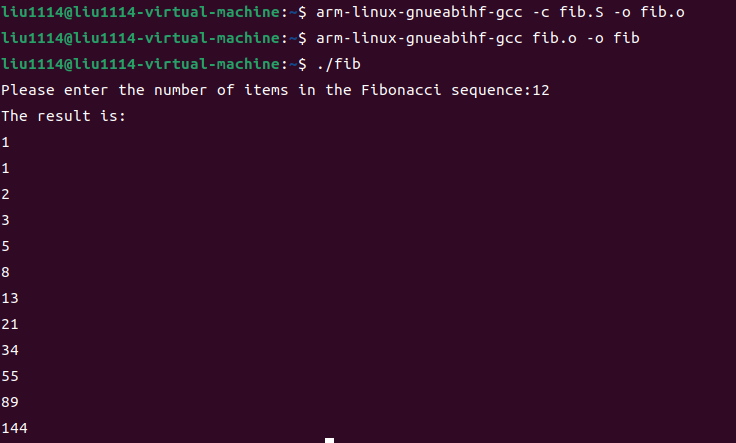
\includegraphics[width=1.0\textwidth]{img/fib_arm.png}
    \caption{fib.S}
\end{figure}
\subsection{阶乘}

\subsubsection{阶乘SysY程序}

sysY语言与C语言类似。
在阶乘的sysY程序中,尽可能地包含了支持的语言特性,设置有全局变量、分支、循环、函数调用等等。
代码如下:
\begin{lstlisting}
#include<stdio.h>

int n=0;  //全局变量

int factorial(int n) {
    int re=1;
    
    if(n>=1)        //分支
    {
        while(n)    //循环
        {
            re*=n;
            n--;
        }
    }
    return re;
}

int main() {
    scanf("%d",&n);         
    int result = factorial(n);   //函数调用
    printf("%d\n",result);
    return 0;
}
\end{lstlisting}

\subsubsection{阶乘ARM汇编程序}


在Ubuntu中编写写好factorial.S文件后,使用命令:


\begin{lstlisting}[frame=trbl]
 arm-linux-gnueabihf-gcc factorial.S -o fac
\end{lstlisting}\par
得到可执行程序fac。

然后使用命令:
\begin{lstlisting}[frame=trbl]
 qemu-arm -L /usr/arm-linux-gnueabihf/ ./fac
\end{lstlisting}\par
运行可执行文件可进行阶乘求解。
如图:
\begin{figure}[H]
    \centering
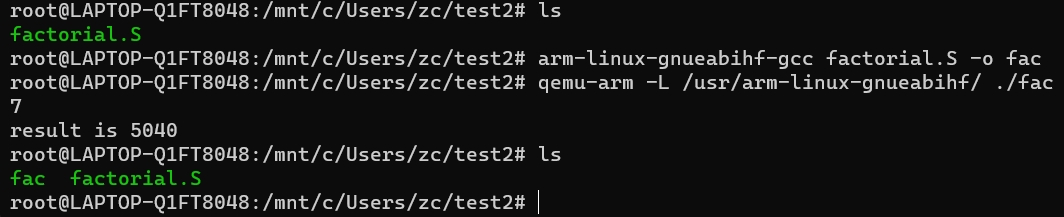
\includegraphics[width=1.0\textwidth]{img/factorial_arm.png}
    \caption{fact.S}
\end{figure}

分别验证0!和12!,结果无误:
\begin{figure}[H]
    \centering
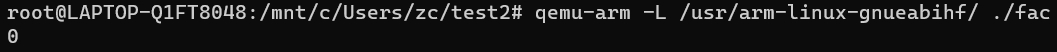
\includegraphics[width=1.0\textwidth]{img/fac_0.png}
    \caption{fac0}
\end{figure}
\begin{figure}[H]
    \centering
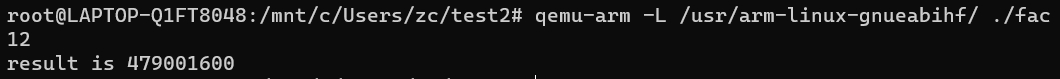
\includegraphics[width=1.0\textwidth]{img/fac_12.png}
    \caption{fac12}
\end{figure}


arm汇编代码如下:
\begin{lstlisting}
    .arch armv7-a      @架构
    .comm a,4          @全局变量a,占4字节
    .text
    .align 2
    .section .rodata
    .align 2
_str0:                 @字符串str0和str1
    .ascii "%d\0"   
    .align 2
_str1:
    .ascii "result is %d\n"
    .text
    .align 2

    .global fac
fac:                    @ 函数 int factorial(int n)
    str fp,[sp,#-4]!    @表示将寄存器 fp 压入栈中,同时更新 sp 指针
    mov fp,sp           @将 sp 指针设置为当前栈指针
    sub sp,sp,#12       @开辟栈空间
    str r0,[fp,#-12]    @ r0 = n
    mov r8,#1           @保存结果
    cmp r0,#1           
    blt .end_fac

.loop:                   @循环
    mul r8,r0            
    sub r0,#1
    cmp r0,#0
    bne .loop
    b .end_fac

.end_fac:
    add sp,fp,#0         @恢复栈空间,恢复寄存器
    ldr fp,[sp],#4
    bx lr                @返回

    .global main
main:
    push {fp,lr}
    add fp,sp,#4
    ldr r1,_bridge     @*r1=n
    ldr r0,_bridge+4   @*r0="%d\n"
    bl __isoc99_scanf
    ldr r3,_bridge     @r3=&n
    ldr r0,[r3]        @r0=n
    bl fac
    mov r1,r8
    ldr r0,_bridge+8   @"result is %d\n"
    bl printf
    mov r0,#0
    pop {fp, pc}

_bridge:
    .word a
    .word _str0
    .word _str1

    .section .note.GUN-stack,"",%progbits    @避免运行时出现的一些问题
    
\end{lstlisting}



\newpage
\bibliographystyle{plain}
\bibliography{references} 
\end{document}
